% 2.2
\section{Den aggregatorienterte datamodellen}

Så har vi den aggregatorienterte modellen, en metamodell som tillater den enkelte systemarkitekt å selv definere kompleksiteten til strukturen til sine egne dataenheter, slik at persisterte data er tilpasset applikasjonens struktur på sine dataobjekter i stedet for å tvinge vedkommende til å konformere med en forhåndsbestemt minste enhet, slik tilfellet er i den relasjonelle modellen. Denne fleksibiliteten i struktureringen av data er et sentralt fellestrekk nøkkelverdilagre som Dynamo og Redis deler med kolonnefamilie-lagre som Cassandra og HBase og dokumentdatabaser som MongoDB og CouchDB. Derfor definerer \cite{sadalage2013} en felles kategori for disse tre NoSQL-typene: ''Aggregatorienterte databasesystem''.

Begrepet ''aggregat'' (må ikke forveksles med det matematiske verbet som betegner en operasjon på en gruppe av tupler) er lånt fra domenedrevet design og er i kontekst av databasemodellering definert som en samling sammenknyttede objekter som en datamodellør ønsker å behandle som en enhet for datamanipulasjon og konsistenshandtering. Når komplekse aggregater aksesseres, gjøres det med et oppslag på én enkelt nøkkel, så får man både dataobjektet med den tilhørende nøkkelen samt eventuelle assosierte dataobjekter. Å utføre en tilsvarende lesing av to assosierte relasjoner i for eksempel MySQL krever først oppslag i en tabell på dens nøkkelverdi, deretter enda et oppslag på en fremmednøkkel i den assosierte tabellen, altså må en JOIN-operasjon utføres. Med begrepet dataobjekt menes en serialisert, distinkt, flatt datastruktur på JSON-form. Et aggregat er til sammenlikning et dataobjekt med nøstede dataobjekter.

En aggregatmodell avgrenser den objektstrukturen til applikasjonens data som alltid skal skrives i ett, hvilket betyr at når data i et nøstet objekt endres, blir hele aggregatobjektet i seg selv omskrevet. Aggregatet utgjør dermed en naturlig enhet for replikering i et distribuert databasesystem, da hele den aggregerte objektstrukturen som programvarens forretningslogikk jobber innenfor, replikeres i sin helhet. En tuppel i en normalisert relasjon inneholder nødvendigvis ikke hele omfanget av dataobjektstrukturen som forretningslogikken opererer med, iallfall ikke uten en eller to JOIN-operasjoner.

% bryt-opp
Aggregatet utgjør også en naturlig enhet for partisjonering. En stor mengde av individuelle aggregater er fra programvaresystemet sitt sitt standpunkt aksessert fullstendig uavhengig av hverandre, derfor kan de fordeles tilfeldig, og kopieres utover et sett med uavhengig opererende databasenoder, uten at objektenes plassering får konsekvenser for applikasjonens aksessmønster - skal en klient ha tak i ett spesifikt objekt kan den i prinsippet kontaktet én spesifikk databasenode i nettverket som er kjent for å holde på dette ønskede objektet. I et relasjonelt, distribuert databasesystem innebærer partisjonering av tabeller negative konsekvenser for spørreytelsen.% TODO: Å partisjonere tabeller i et   påvirke ytelsen til forskjellige spørringer etter forskjellige tupler som tilhører samme tabell, på grunn av algoritmen den distribuerte JOIN-operasjonen er implemntert med så vel som plasseringen av tupler med matchende assosiasjonsvariable (lik verdi for fremmednøkkel og primærnøkkel).  bryt-opp  , avhengig av de rådende assosiasjoner og fremmednøkkelbegrensninger,

% bryt-opp
Lesing av aggregerte dataobjekter medfører at man med ett enkelt oppslag på én enkel nøkkel får både i pose og sekk. Aggregatmodellen er også en enklere datamodell å forholde seg til for de som programmerer selve applikasjonen som behandler dataene, av den enkle grunn at de slipper å skrive kode for å konvertere en tilfeldig liste av flate tupler. De enkelte aggregater, det vil si applikasjonsprogrammererens definisjon for databehandlingsenhet utgjør en naturlig enhet for replikering i en klynge av enkeltstående databasenoder. I et distribuert databasesystem gjelder det å minimalisere antall noder som kontaktes for hver spørring. Når konsepter settes sammen eksplisitt i datamodellen slik som vi ser i de fleksible dokumentstrukturene til Mongo, vet databasen hvilke dataenheter som skal aksesseres samtidig, og som derfor naturlig nok bør plasseres på én og samme node.

\cite{sadalage2013} kaller relasjonelle databaser og grafdatabaser for \textbf{aggregat-uvitende}. Deres datamodeller betrakter ikke aggregater eller sammensatte datastrukturer i deres dataoperasjoner. Aggregat-uvitenhet er ikke nødvendigvis et dårlig designvalg, ettersom det ikke alltid er opplagt for den enkelte webapplikasjonsutvikler hvilke enhetsbegrensinger i datamodellen som er logiske, iallfall ikke før datamodellen er definert for første gang og revidert to til tre ganger i løpet av utviklingsprosessen. Den lagrede dataen kan ha mange forskjellige brukskontekster, avhengig av applikasjonens funksjonelle krav som ofte blir forandret underveis i applikasjonens livssyklus.

En enkelt aggregatstruktur kan ikke medføre optimale spørringsytelse for alle mulige brukskontekster. Her gjelder det for utvikleren å prioritere den mest typiske leseoperasjonen tjenesten utsettes for. Hvis applikasjonen ikke har en slik primær aksess – struktur på dataobjektene kan man like godt modellere dem på et aggregat-uvitende vis. I en aggregat-uvitende modell har brukskonteksten ingen innvirkning på spørringen, fordi operasjonsenheten er én enkelt tuppel i MariaDB uansett hvordan konseptene er satt sammen.

Aggregatorienterte databasesystemer innehar ikke ACID - egenskapene som vi finner hos transaksjoner i relasjonelle databasesystemer. Imidlertid støtter de naturlig atomiske manipulasjoner på ett eneste aggregat av gangen. Ved nøkkeloppslag får man hele dataobjektet den tilkoplete applikasjonen leser og manipulerer, Samtidighetskontroll ved operasjoner på flere aggregater må følgelig handteres i kildekoden til applikasjonen, spørring for spørring, der et unntak må kastes hvis én av spørringene mislykkes. Å emulere transaksjoner i enkeltaggregater inngår som en viktig faktor i hvordan aggregatene defineres i datamodellen \citep{sadalage2013}.

% 2.2.1
\subsection{Design av aggregatmodeller}

Slik kan en generisk aggregatmodell, uttrykt i UML, ekvivalent til datamodellen fra \ref{fig1} se ut.

% Figur 2
\begin{figure}[!ht]
    \centering
    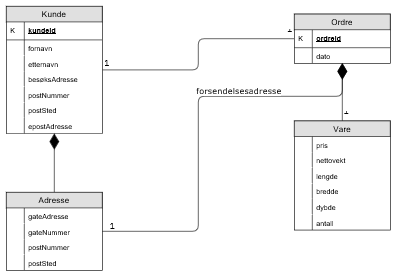
\includegraphics[scale=0.7]{fig/NettbutikkAggregatModell.png}
    \caption{Aggregatdiagram med to forskjellige entiter, modellert for den samme tjenesten fra \ref{fig1}.}
    \label{fig2}
\end{figure}

Denne figuren presenterer to forskjellige aggregatmodeller, \texttt{Kunde} og \texttt{Ordre}. \cite{sadalage2013} demonstrerer et eksempel på en aggregatorientert modell i samme forretningsdomene, med de samme to entitetene. Forbindelsen mellom disse to denoterer en én-til-mange-assosiasjon som man kjenner til fra den relasjonelle modellen, men som ikke realiseres med fremmednøkler, iallfall ikke fremmednøkler slik man er vant til dem fra MySQL og PostgreSQL. I stedet indikerer denne assosiasjonen i diagrammet at hvert kundeaggregat har en flat liste bestående av \texttt{Ordre}-nøkler som representerer alle ordrene en kunde har opprettet i netthandelen. Likeledes kan hver enkelt ordre holde på en ''fremmednøkkel'' som kun applikasjonen kan tolke, og således er det i selve applikasjonslogikken av nettbutikksystemet at ''JOIN'' blir gjort. Komposisjonselementet indikerer bruk av nøsting i aggregatet, det vil si at et Vare-objekt til enhver tid eksisterer innenfor et aggregat, nemlig \texttt{Ordre}-entiten, og aldri som et selvstendig aggregat selv. I relasjonelle ER-modeller er slik nøsting av entiteter strengt forbudt. Aggregatorienterte modeller er således \emph{denormaliserte}, det vil si at den enkelte aggregatmodell ikke oppfyller første normalform.

1NF-relasjoner består av flate tupler uten nøsting av relasjoner, eller som \cite{codd1971} definerer en unormalisert tabell: ''[a] group schema which contains a repeating group schema''. Med ''repeating group'' menes også attributter på listeform, for eksempel en liste av strenger. Videre tillater ikke \cite{codd1971} kryssreferanse per primærnøkkel innad i en relasjon, fordi det er en uønsket egenskap for en relasjon å ha, datamodellen blir følgelig rotete og vanskelig å lese for dens brukere.

En annen interressant detalj ved modellen presentert i \ref{fig2} er at Adresse-objektet er inneholdt i både \texttt{Kunde}-aggregatmodellen og \texttt{Ordre}-aggregatmodellen. Semantikken bak er at hver ordre har en leveringsadresse som de tilknyttede varene leveres til. I praksis betyr dette at aggregater av både \texttt{Ordre} og \texttt{Kunde} lagrer potensielt samme adresseinfo, altså er adressedataobjekt lagret dobbelt opp i databasen, den er \emph{duplisert}.

% bryt-opp
Ved modellering av aggregater må man avveie mellom hvor stort hvert enkelt aggregatobjekt i en applikasjon kan bli og hvor mange forskjellige aggregatentiter applikasjonen kan ha. Alternativt kunne datamodellen i \ref{fig2} bestått av ett eneste aggregat, noe man oppnår ved å erstatte assosiasjonslinjen mellom \texttt{Kunde} og \texttt{Ordre} med en komposisjonslinje. Med to nivåer av nøstede lister av objekter innen ett aggregat, kan besvarelse av ett enkelt oppslag på én spesifikk nøkkel potensielt medføre et så stort svar i retur at HTTP-responsen må deles opp i flere TCP-pakker, hvilket igjen er delt opp i mange IP-pakker som tar forskjellige ruter til den spørrende klienten. Store, komplekse aggregat vil innvirke på spørringens nettverksforsinkelse. \cite{sadalage2013} poengterer at hvis applikasjonen alltid har bruk for å hente informasjon om ordre, samtidig som den henter informasjon om en kunde, så er det hensiktsmessig å legge ordrehistorikken til hver kunde inn under Kunde-aggregatet. Hvis applikasjonen fokuserer på kun én ordre ad gangen i dets brukervisning, så vil todelingen av aggregater som vist i \ref{fig2} være mer hensiktsmessig. Hvordan aggregater defineres er alt i alt opp til den enkelte datamodellør.

% Skriv om tre ulike aggregat - orienterte datamodeller - Segway til påfølgende delkapitler
Fowler og Sadalage omtaler tre unike datamodeller som opererer med aggregater. Nøkkelverdimodellen behandler det enkelte aggregat som en ugjennomsiktig helhet \citep{sadalage2013}. Altså går det ikke an å hente deler av aggregatet ved et nøkkeloppslag. Dokumentmodellen eksponerer aggregatet til databasen, og tillater dermed delvise spørringer. I og med at dokumentmodellen også er skjemaløs, går det ikke an å optimalisere spørringer på hele eller deler av aggregatet. Kolonnefamilier inndeler aggregatet i grupper, noe som tillater databasen å operere på hver av disse gruppene som en egen dataenhet, liksom attributter i tuplene i den relasjonelle modellen. Selv om kolonnefamilier til dels ofrer den komplette skjemaløsheten som vi ser i nøkkelverdimodellen, har databasen nå mulighet til å nytte eksponeringen av attributter/kolonner til å optimalisere aksesseringer og oppdatere separate kolonner.

% 2.2.2
\subsection{Nøkkelverdimodellen}

Nøkkelverdi-lagre er den type NoSQL-DBMS med den enkleste aggregatorienterte datamodellen. Dens hovedkarakteristikk er at hvert aggregat som lagres må være tilknyttet én unik identifikator kalt \textbf{nøkkel}, og for å hentet det lagrede aggregatet må man vite verdien til denne nøkkelen \citep{elmasri2014}. En nøkkel er en helt unik streng som brukes av databasesystemet til å lokalisere raskt et assosisert dataobjekt (også kalt \textbf{verdi}) i en homogen klynge av databasenoder \citep{elmasri2014}. Hvert aggregat som lagres er ugjennomsiktig, det er en stor boble av serialiserte bytes som databasesystemet ikke kan anskue. I prinsippet er nøkkelverdimodellen totalt ustrukturert, altså er det opp til selve applikasjonen hvis data lagres i nøkkelverdidatabasen å påføre dataobjektet mening og definere dets struktur \citep{elmasri2014}. Fordelen med at aggregatet ikke synes i databasen er at applikasjonsutvikleren kan endre aggregatets struktur, også kjent som dets implisitte skjema, helt etter eget ønske. Man kan lagre hva man enn vil i et nøkkelverdilager så lenge man spesifiserer en nøkkel databasen bruker til å lete opp dataobjektet med, og følger en eventuell størrelsesbegrensning definert av databasens konfigurasjon \citep{sadalage2013}.

Spørringer skrives ikke i et domenespesifikt språk som for eksempel SQL. I stedet kaller applikasjonen på et sett funksjoner eksponert for den gjennom et applikasjonsprogrammeringsgrensesnitt (API). Dette APIet tilbyr hovedsaklig tre forskjellige spørringer: Lesespørring (\texttt{GET}), skrivespørring (\texttt{PUT}) og slettespørring (\texttt{DELETE}). Både oppdateringer og opprettelser av dataverdier gjøres med én og samme kommando, PUT. Enkelte nøkkelverdidatabaser kan supplere med flere funksjoner til for eksempel administrative behov. Hver enkelt spørring behandler \underline{ett helhetlig aggregat av gangen}. En lesespørring på en nøkkel henter ut hele aggregatobjektet assosiert med nøkkelen. En skrivespørring som oppdaterer et dataobjekt skriver over eksisterende data assosiert med objektets nøkkel fullstendig.

Moderne, populære NoSQL-systemer avviker noe fra dette prinsippet som skiller nøkkelverdimodellen fra dokumentmodellen. I dokumentlagre går det an å definere et ID-felt, en primærnøkkel, brukt til å gjøre ID-oppslag på samme vis som i et nøkkelverdilager. Riak KV tillater applikasjonsutvikleren å legge inn metadata direkte inn i det lagrede aggregatobjektet slik at deler av aggregatet indekseres, og det samme systemet implementerer også en form for assosiasjon mellom aggregater. Videre har Riak også en søkefunksjon som kan brukes på JSON-serialiserte aggregater \citep{sadalage2013}. Redis, et annet nøkkelverdisystem, støtter lagring på og oppslag av aggregatobjekter som ikke likner på tradisjonelle JSON-objekter, men objekter i form av lister, hashede verdier og mengder.

% bryt-opp
I kraft av databasens egenskap i å støtte kun én eneste indeks, nemlig oppslagsnøkkelen til dataobjektene, er nøkkelverdimodellen forenlig med systemkrav om at datavolumet som lagres skal jevnfordeles utover en klynge av uavhengig opererende databasenoder. Å ta høyde for aggregateksponering til datalageret, direktereferanser til andre aggregat, og delvis indeksering på aggregatet, gjør oppfyllelse horisontal skalerbarhet i databasen vanskeligere. Videre er kontroll av transaksjonskonsistens (også kjent som ''Consistency'' i ACID-forkortelsen) en jobb som i utgangspunktet ''outsources'' til applikasjonen, fordi nøkkelverdi-lageret er prinsipielt uvitende om den bakenforliggende semantikken til det enkelte dataobjekt.

% 2.2.3
\subsection{Dokumentmodellen}

I motsetning til nøkkelverdilagre er det enkelte aggregatobjekt sin datastruktur synlig for dokumentlagre, som også kan utføre både lesespørringer og oppdateringsspørringer på spesifikke feltvariable innen de lagrede aggregater, altså bare hente ut distinkte deler av dokumenter. Dokumentlageret kan lese av disse ''selvbeskrivende dataene'' \citep{sadalage2013, elmasri2014} som finnes i aggregatobjektene, og derfor er slike delvise spørringer mulig. De enkelte attributter/feltvariable innen aggregater som er interressant for en applikasjon kan også indekseres av databasen på samme måte som relasjonsdatabaser er i stand til å indeksere enkeltattributter i relasjoner. Samtidig fører dokumentlageret begrensninger på hvordan strukturen til det lagrede aggregatet kan se ut, gjennom definisjoner av tillatte datatyper og objektstrukturer \citep{sadalage2013}. På tross av at dokumentdatabasen kan anskue aggregatets struktur opererer hver enkelt spørring på ett enkelt, helhetlig dokument av gangen.

Dokumentlagere inndeler vanligvis data i samlinger (eng. ''collections'') av dokumenter (eng. ''documents''). De enkelte dokumenter er aggregatobjekter utformet i et semistrukturert format, som XML eller JSON. Dokumenter lagret innen samme dokumentsamling tillates å ha forskjellige definerte eller udefinerte verdier for enkelte variable. Denne fleksible egenskapen er ikke å finne i den relasjonelle modellen.

Spesifikt i MongoDB lagres dokumenter i BSON, et binært format som er en utvidelse av JSON-standarden med noen ekstra datatyper, optimalisert for lagring på disk. For å opprette en ny dokumentsamling har MongoDB metoden \texttt{createCollection}, som tar inn samlingens navn og en mengde innstillinger som bestemmer begrensninger for samlingen, som for eksempel det totale datavolumet og det maksimale antallet dokumenter som samlingen kan holde på. Hvert dokument har et automatisk generert felt som MongoDB bruker som primærnøkkel, med mindre applikasjonsutvikleren definerer en slik indeks selv \citep{elmasri2014}.

Dokumentsamlinger er ikke bundet til et skjema slik som relasjonelle databaser. Strukturen til aggregatet/dokumentet defineres av applikasjonens utviklere, og velges utifra applikasjonens krav til datamodellen, i stedet for at appliaksjonens logikk tilpasser seg en rigid, todimensjonal struktur slik vi ser i relasjoner. Følgelig blir det umulig for databasesystemet å optimalisere spørringer med basis i aggregatstrukturen, fordi den er ikke gitt før innsettingsspørringer tikker inn (i kontekst av Mongo via \texttt{insert} - funksjonen).

% 2.2.4
\subsection{Kolonnefamiliemodellen}

Googles BigTable er et databasesystem som har inspirert mange senere NoSQL-systemer, akkurat som Dynamo. BigTable er en ofte brukt lagringsteknologi hos Googles applikasjoner, deriblant Gmail \citep{elmasri2014}. Apache HBase er et kolonnefamilielager tilgjengelig i åpen kildekode\footnote{Tilgjengelig på følgende GitHub-repositorium: \url{https://github.com/apache/hbase}} som implementerer de sentrale teknikkene inneholdt i BigTable.

Kolonnefamilielagre kan beskrives av \cite{elmasri2014} som ordnede, flerdimensjonale, distribuerte ordlister, hvorav nøkkelverdilagre som Redis kan ansees å være enkeltdimensjonale, distribuerte ordlister. Den enkelte aggregat-nøkkel i et kolonnefamilielager består av flere distinkte komponenter, vanligvis et navn på samlingen av aggregater, en nøkkel som identifiserer selve aggregatet (''row key''), aggregatet i seg selv som også refereres til som en ''kolonne'' og et tidsstempel \citep{elmasri2014}.

\newpage

% Figur 3
\begin{figure}[!ht]
    \centering
    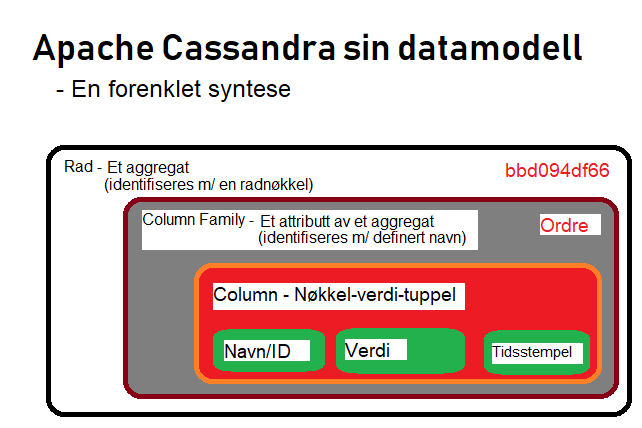
\includegraphics[scale=0.7]{fig/kolonneorientert.png}
    \caption{Metamodell som viser forholdene mellom dataenheter i Cassandras logiske datamodell.}
    \label{fig3}
\end{figure}

I et kolonnefamilelager er hvert enkelt aggregat identifisert av en todimensjonal nøkkel: Den ene komponenten er en radnøkkel og den andre er navnet på en kolonnefamile underordnet ''raden'', som i Cassandra er en samling aggregater (se \ref{fig3}). En kolonnefamilie er en samling nøkkel-verdi-tupler, ikke ulikt en tuppel og dens attributter i den relasjonelle datamodellen.

I eksempelet i \ref{fig2} med aggregatmodellen måtte man i de øvrige to datamodellene velge mellom å ha èn entitet, Kunde med \emph{n} Ordre underordnet, eller to altså at lesing av kundedata innebærer raskere lesing på disk, men innhenting av alle ordre må gjøres med \emph{n} enkeltoppslag når listen av ordreID-er i kundens ordreliste er av størrelse \emph{n}. I et kolonnefamilielager kan man i prinisppet få i pose og sekk ved å definere hvert aggregat til å representere en kunde og la samlingen av \texttt{Ordre}-entiteter underordnes som en kolonnefamilie i tillegg til å definere en annen kolonnefamilie, Profil, som inneholder kundens personlige data og leveringsadresse. Hvis applikasjonen nå er interresert i en kundes profildata, slipper den å hente alle dens ordre i tillegg.
